\documentclass[11pt, oneside]{article}
\usepackage[bottom=2.5cm,top=2.5cm]{geometry}
\geometry{a4paper}
\usepackage{graphicx}
\usepackage{amssymb}
\usepackage[utf8]{inputenc}
\usepackage[brazil]{babel}
\usepackage{color}
\usepackage{float}
\usepackage{hyperref}
\bibliographystyle{apalike}
\usepackage{indentfirst}

\title{Briefing Clima Espacial}
\date{25/04/2022}

\begin{document}
\maketitle 

 \section{ROTI} 
 \subsection{Responsible: Carolina de Sousa do Carmo} 
 
\begin{figure}[H]
    
                        \centering
   
                             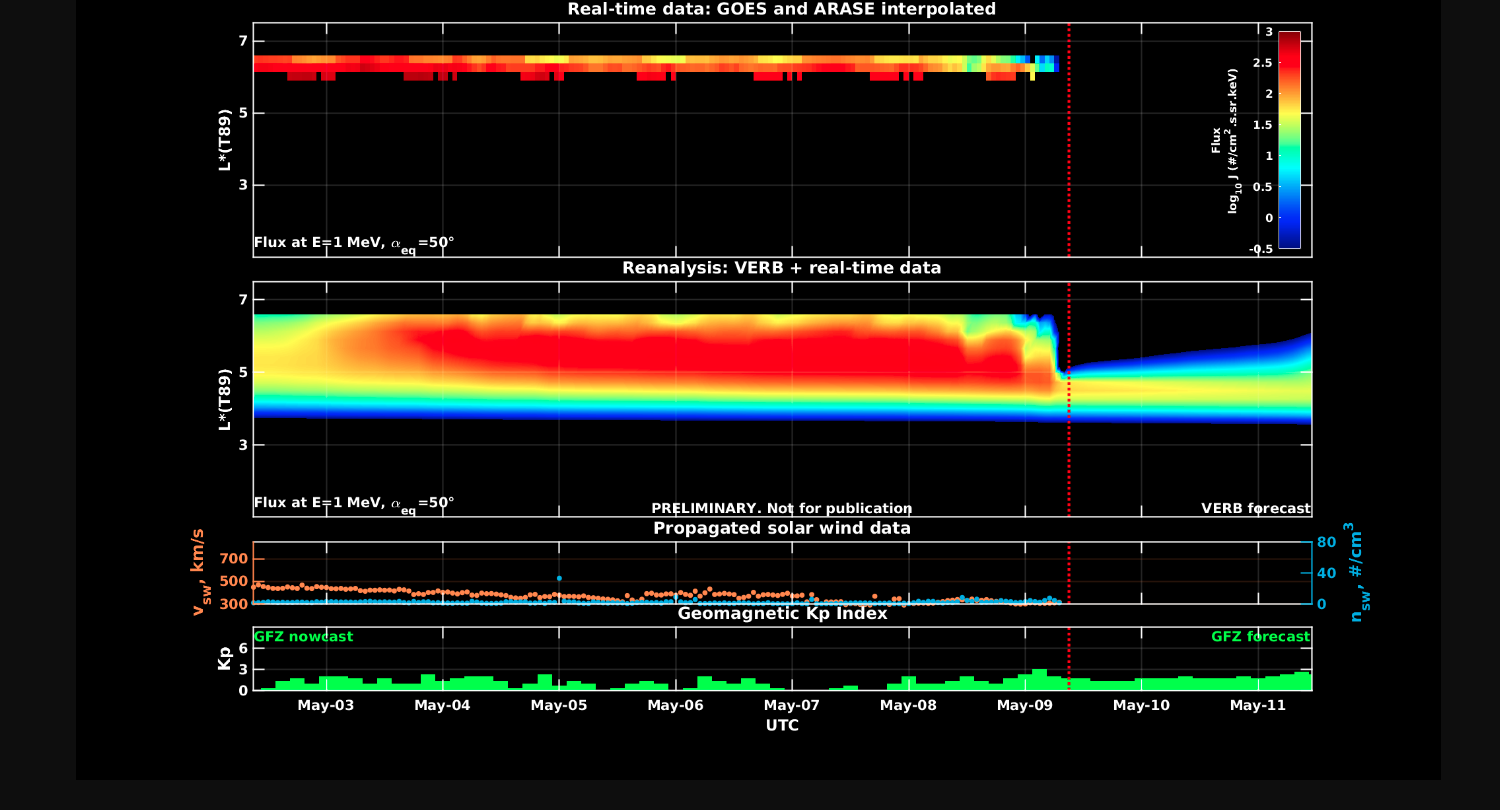
\includegraphics[width=14cm]{./figures/figureRadBelts_1.png}

                             \caption{Figure 1 - Keogram of the ROTI index for fixed geographic latitudes 5°S and 15°S, on April 25, 2022.}
                        \end{figure}

                     \begin{figure}[H]
    
                        \centering
   
                             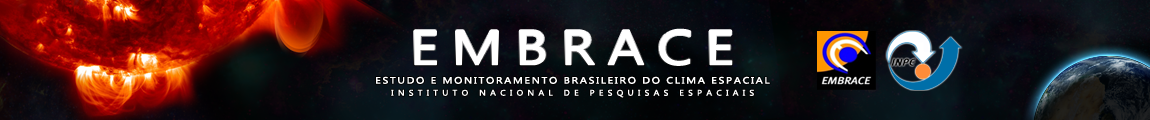
\includegraphics[width=14cm]{./figures/figureRadBelts_2.png}

                             \caption{Figura 1 – Keograma do índice ROTI, para as latitudes geográficas fixas 5°S e 15°S, do dia 25 de abril de 2022.}
                        \end{figure}

                     

Carolina de Sousa do Carmo



O ROTI (“Rate of TEC index”) é um índice baseado na variação do TEC (“Total Electron Content”) (Pi et al., 1997). Este índice é utilizado na detecção de irregularidades ionosféricas, como as bolhas de plasma. O índice ROTI apresenta boa correlação com o índice de cintilação S4 (e.g., Carrano et al., 2019). A Tabela 1 mostra o resumo da semana (24-30 de abril de 2022) de acordo com o índice ROTI, evidenciando os horários de detecção de irregularidades ionosféricas no setor da América do Sul. Em seguida, as Figuras 1 mostra os keogramas do índice ROTI, para as latitudes geográficas fixas 5°S e 15°S, com longitude geográfica versus hora universal (UT).



Tabela 1 – Resumo da semana (24-30 de abril de 2022).



Figura 1 – Keograma do índice ROTI, para as latitudes geográficas fixas 5°S e 15°S, do dia 25 de abril de 2022.



Em resumo, os dias 25 e 26 de abril tiveram estruturas similares a bolhas de plasma, nos horários indicados na Tabela 1, na região norte do Brasil. Porém, essa região possui baixa cobertura de receptores GNSS facilitando a propagação de erros e efeito de bordas nos mapas.




\end{document}